% Bagian Lampiran
\section*{Lampiran} % Jika ada lampiran
\begin{figure}[H]
  \centering
  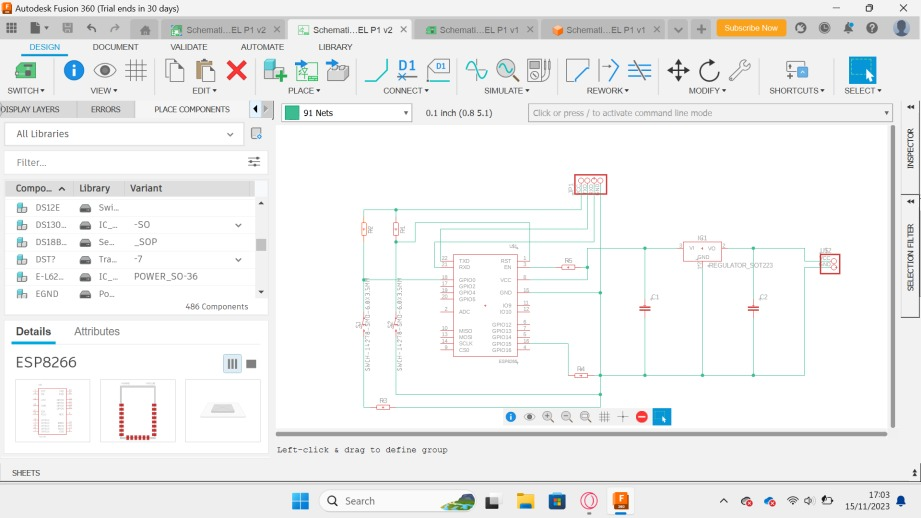
\includegraphics[width=0.7\linewidth]{img/modul_1/schematic.jpg}
  \caption{Membuat schematic} 
  \label{fig:inirujukan}
\end{figure}
\vspace{0pt}
\begin{figure}[H]
  \centering
  % Kalau mau menambah gambar lagi tinggal nambahin begin{subfigure} -> end{subfigure}
  \begin{subfigure}[b]{0.4\linewidth}
    \centering
    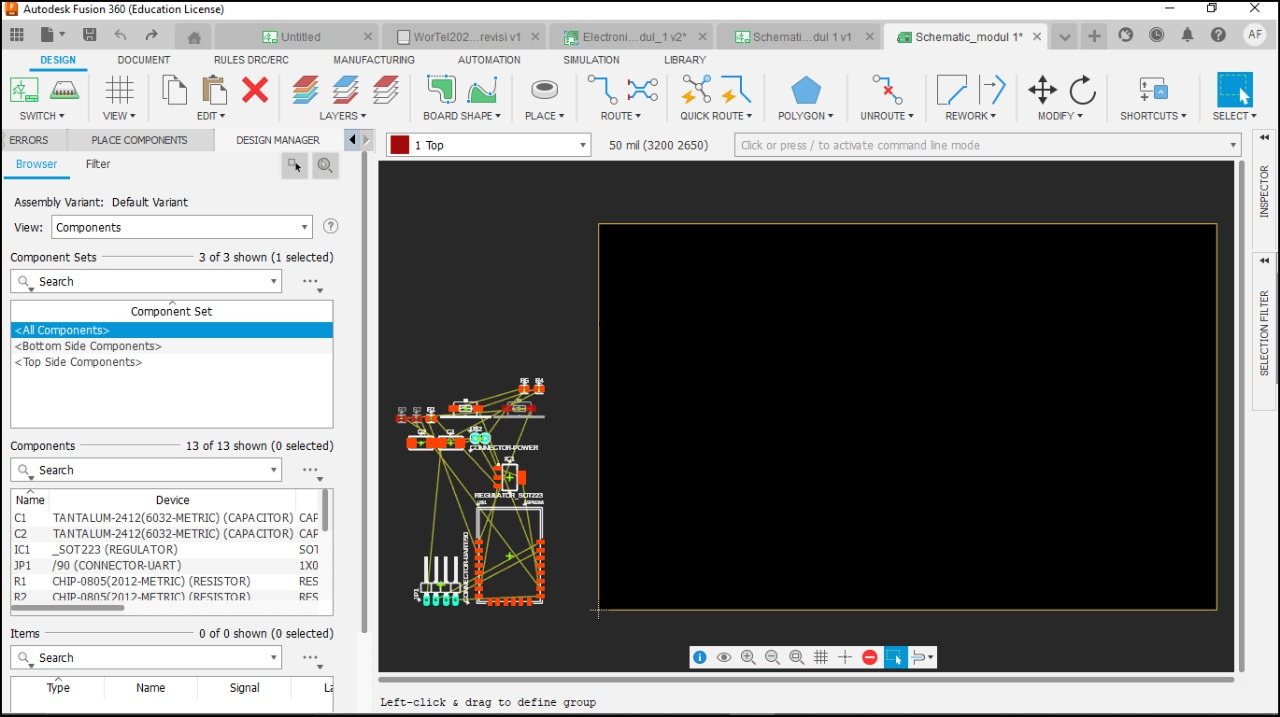
\includegraphics[width=\linewidth]{img/modul_1/circuit before1.jpeg}
    \caption{Komponen PCB sebelum dirangkai\label{fig:inisub1}}
  \end{subfigure}
  \hspace{1cm}
  \begin{subfigure}[b]{0.4\linewidth}
    \centering
    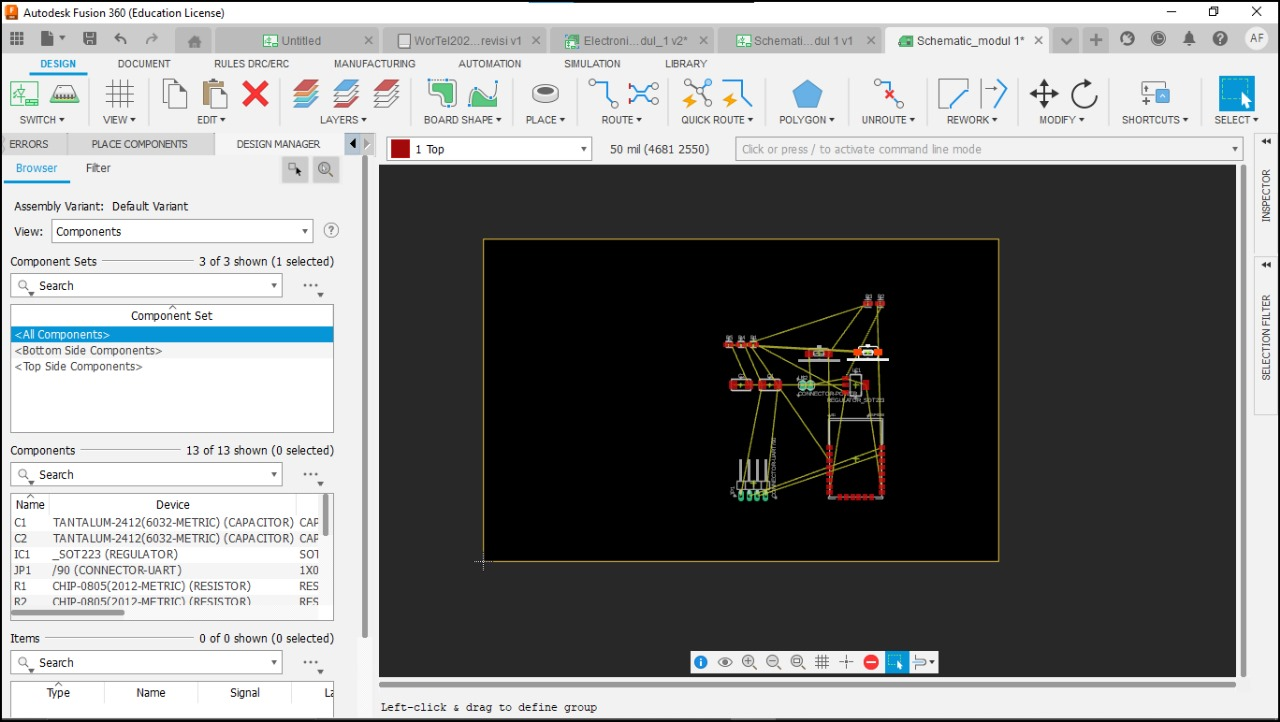
\includegraphics[width=\linewidth]{img/modul_1/circuit before.jpeg}
    \caption{Mulai merangkai PCB\label{fig:inisub2}}
  \end{subfigure}
  \caption{Proses merangkai PCB\label{fig:keduagambar}}
\end{figure}

\begin{figure}[H]
  \centering
  % Kalau mau menambah gambar lagi tinggal nambahin begin{subfigure} -> end{subfigure}
  \begin{subfigure}[c]{0.4\linewidth}
    \centering
    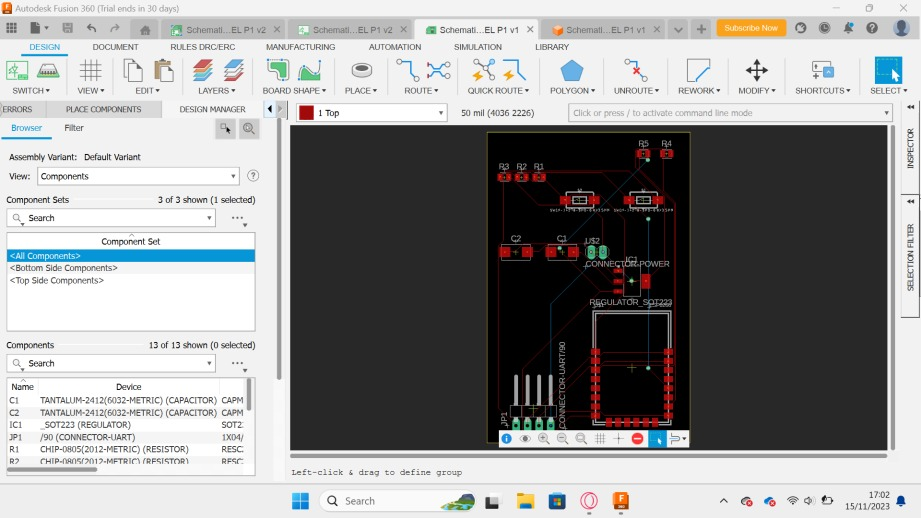
\includegraphics[width=\linewidth]{img/modul_1/PCB DONE.jpeg}
    \caption{Routing complete\label{fig:inisub1}}
  \end{subfigure}
  \hspace{1cm}
  \begin{subfigure}[c]{0.4\linewidth}
    \centering
    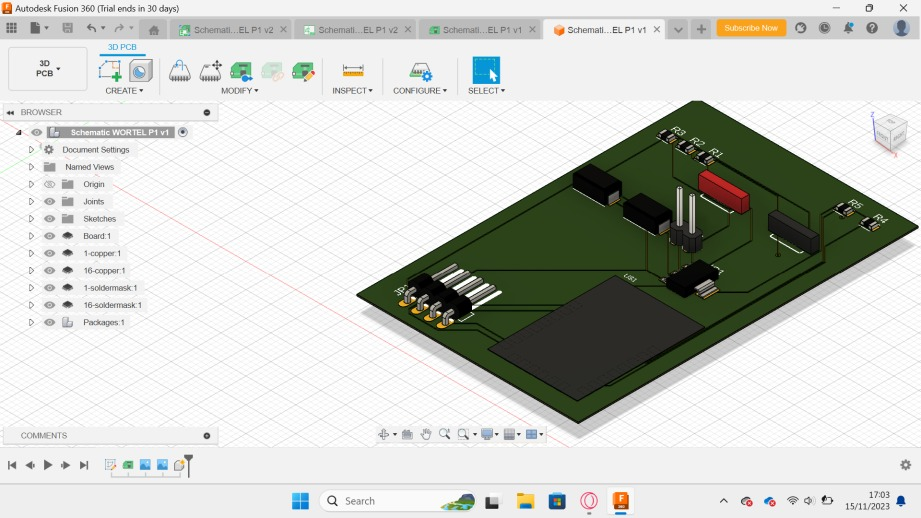
\includegraphics[width=\linewidth]{img/modul_1/3D Model.jpeg}
    \caption{visualisasi 3D dari PCB\label{fig:inisub2}}
  \end{subfigure}
  \caption{Hasil\label{fig:keduagambar}}
\end{figure}